\documentclass{article}

\usepackage{amsmath}

\usepackage[dvips]{graphicx}

\renewcommand{\vec}[1]{\boldsymbol{#1}}

\begin{document}

\title{A Bayesian introduction to statistical classification}

\author{Peter Mills}

\maketitle

\section{Introduction}

\begin{figure}
	\includegraphics[width=0.9\textwidth]{sample_class}
	\caption{A sample statistical classification problem, showing the border between the two classes.}
\end{figure}

Probability theory is one of the most fundamental tools we have for describing the universe. It is especially relevant to statistical classification and can be used to derive a multitude of important results and to inform our understanding.
This introduction is intended to help you understand probability theory and Bayes� theorem and how they apply to statistical classification. It will allow you to derive non-obvious results that can vastly improve and simplify your classification models.

Note that this introduction, while intended for beginners, nonetheless assumes
knowledge of first- and some second-year university-level mathematics, 
especially linear algebra but also some single and multi-variate calculus.
If the equations seem confusing at times, try to focus instead on 
solving real problems.
You will learn a whole lot more about probability and statistical 
classification by working through some examples than by reading about it
or browsing equations.
For this reason we have provided a set of problems at the end of the article.

\section{Review of basic probability}

Suppose we role a die. There will be six possibilities, each of which
(in a fairly loaded die) will have a probability of 1/6.
We can write this:
\begin{equation}
	P_i = 1/6
\end{equation}
where $i$ is the number on the top side of the die.
Since at least one side will have to come up, we can also write:
\begin{equation}
	\sum_{i=1}^n P_i = 1
\end{equation}
where $n=6$ is the total number of possibilities.

Now suppose we roll two dice. 
The joint probability of getting one of 36 pairs of numbers is given:
\begin{equation}
	P_{ij} = 1/36
\end{equation}
where $i$ is the number on the first die and $j$ that on the second.

If we ignore the number on the second die, the probability of getting a
certain number (a six, say) on the first die is given:
\begin{equation}
	P_i = \sum_i P_{ij} = 1/6
	\label{prior_prob}
\end{equation}
This is known as the prior probability.

Here's where things start getting more complicated.
What is the probability of getting a certain number on one die given that
 a certain number on the other die has come up?
In this case, the two events are uncorrelated, thus the value, at 1/6, will
always be the same but this need not be the case.

Consider a game of Black Jack.
What is the probability that the next card drawn is worth ten points (is a ten
or a face card) given that the previous card was also worth ten points?
Suppose there were 7 ten-point cards out of a deck of 34 remaining before
the last draw.
Now the probabilities are different depending upon the outcome of the previous
event.
If the previous card was worth ten, there is a $6/33=2/11$ chance of getting a card
worth ten, otherwise the probability is $7/33$.
Since the probability that the previous card was worth ten is $7/34$
the joint probability, or the probability of both event occuring is:
\begin{equation}
	P_{ij} = P(j | i) P_i = (7/34)(2/11) = 7/187 \approx 0.0374
	\label{joint_prob}
\end{equation}
where $P_i$ is the probability that the previous cards was worth ten and
$P(j|i)$ is the conditional probability that the next card will be worth ten
given that the previous card was also worth ten.

With prior, joint, and conditional probabilities defined, we are set to write
down Bayes theorem.
Note that these definitions are symmetric in $i$ and $j$, thus:
\begin{equation}
	P_{ij} = P(j|i) P_i = P(i|j) P_j
	\label{Bayes_thm}
\end{equation}
which is the symmetric form of Bayes theorem.

\section{Continuous probabilities}

The extension to continuous probabilities or {\it probability densities} is
straight forward.
Suppose we have a random variable, $x$, governed by a probability distribution,
$P(x)$.
The probability that $x$ takes on a value between $x_0$ and $x_0+\mathrm d x$ is
given:
\begin{equation}
	\lim_{\mathrm d x \rightarrow 0} \left \lbrace \mathrm{Prob}(x_0 \le x \le x_0+\mathrm d x) = \mathrm d x P(x_0) \right \rbrace
	\label{density}
\end{equation}
When working with continuous random variables, summations become integrals
so that Equation (\ref{prior_prob}) becomes:
\begin{equation}
	P(x) = \int P(x,\, y) \mathrm d y
\end{equation}
where the $P(x,\,y)$ is the joint probability of both $x$ and $y$ and the 
integral is over the domain of $x$.

In statistical classification, we are dealing with probabilities
having a very specific form.
One of the variables is scalar and discrete while the other is vector
and continuous. Thus:
\begin{equation}
	P(\vec x, \, i) = P (i|\vec x) P(\vec x) = P(\vec x|i) P(i)
\end{equation}
where $i$ is the class or {\it class label} and $\vec x$ is a vector of 
attributes or {\it features}.

Typically, the goal of Bayesian-based statistical classification is to
estimate either the joint probability, $P(\vec x, \, i)$, or the conditional
probability, $P(\vec x| i)$.
Classifications are normally done on the basis of {\it maximum likelihood}:
\begin{equation}
	c (\vec x) = \arg \max_i P(i|\vec x) = \arg \max_i P(\vec x,\, i)
\end{equation}
where $c$ is the most likely estimate for the class, that is the index
of the largest value of the conditional probability.
Note that because $P(\vec x)$ is the same for a given test point, using
either the joint or conditional probabilities will produce the same result.
The conditional probabilities of the feature space given the class, 
$P(\vec x|i)$, are important also as these 
describe the distributions of each isolated class: that is, if you remove all 
other class labels leaving only $i$, this is the distribution you are left with.

We can use the definition of probability density in (\ref{density}) to derive one of the oldest and
most sophisticated statistical classification technique by simply removing
the limit sign.
Consider picking a radius from the test point, $\vec x$, then
counting the number of training samples of one class or another within
that distance.
The problem with this is that sometimes the enclosed volume will contain 
no samples while other times it may contain a great many.
So rather than distance, we instead fix the number of samples and implicitly
choose the distance on this basis.
This is what is known as a {\it $k$-nearest-neighbors} (KNN) classifier where $k$
is the number of neighboring samples used in each classification.


\section{Binary classifiers}

A binary classifier is special because you can, in many cases, draw a single
hyperplane in the feature space that separates the two classes.
A hyperplane is a sub-space having dimension one less than the embedding 
dimension.
So for a two-dimensional feature space the boundary would be a line while in
three-dimensions, a plane.

Most binary classifiers return not an integer having only two values, but
a continuous, {\it decision function}.
A convenient form of the decision function would be the difference in
conditional probabilities:
\begin{equation}
	R(\vec x) = P(+1|\vec x) - P(-1|\vec x)
	\label{decision}
\end{equation}
where, for convenience, we have chosen the class values to be $-1$ and $+1$.
Unfortunately most statistical classifiers {\it do not} return a decision
function that estimates this quantity well
so a significant chunk of the rest of this article will be dedicated
towards describing methods of calibrating it so that it does.

\begin{figure}
	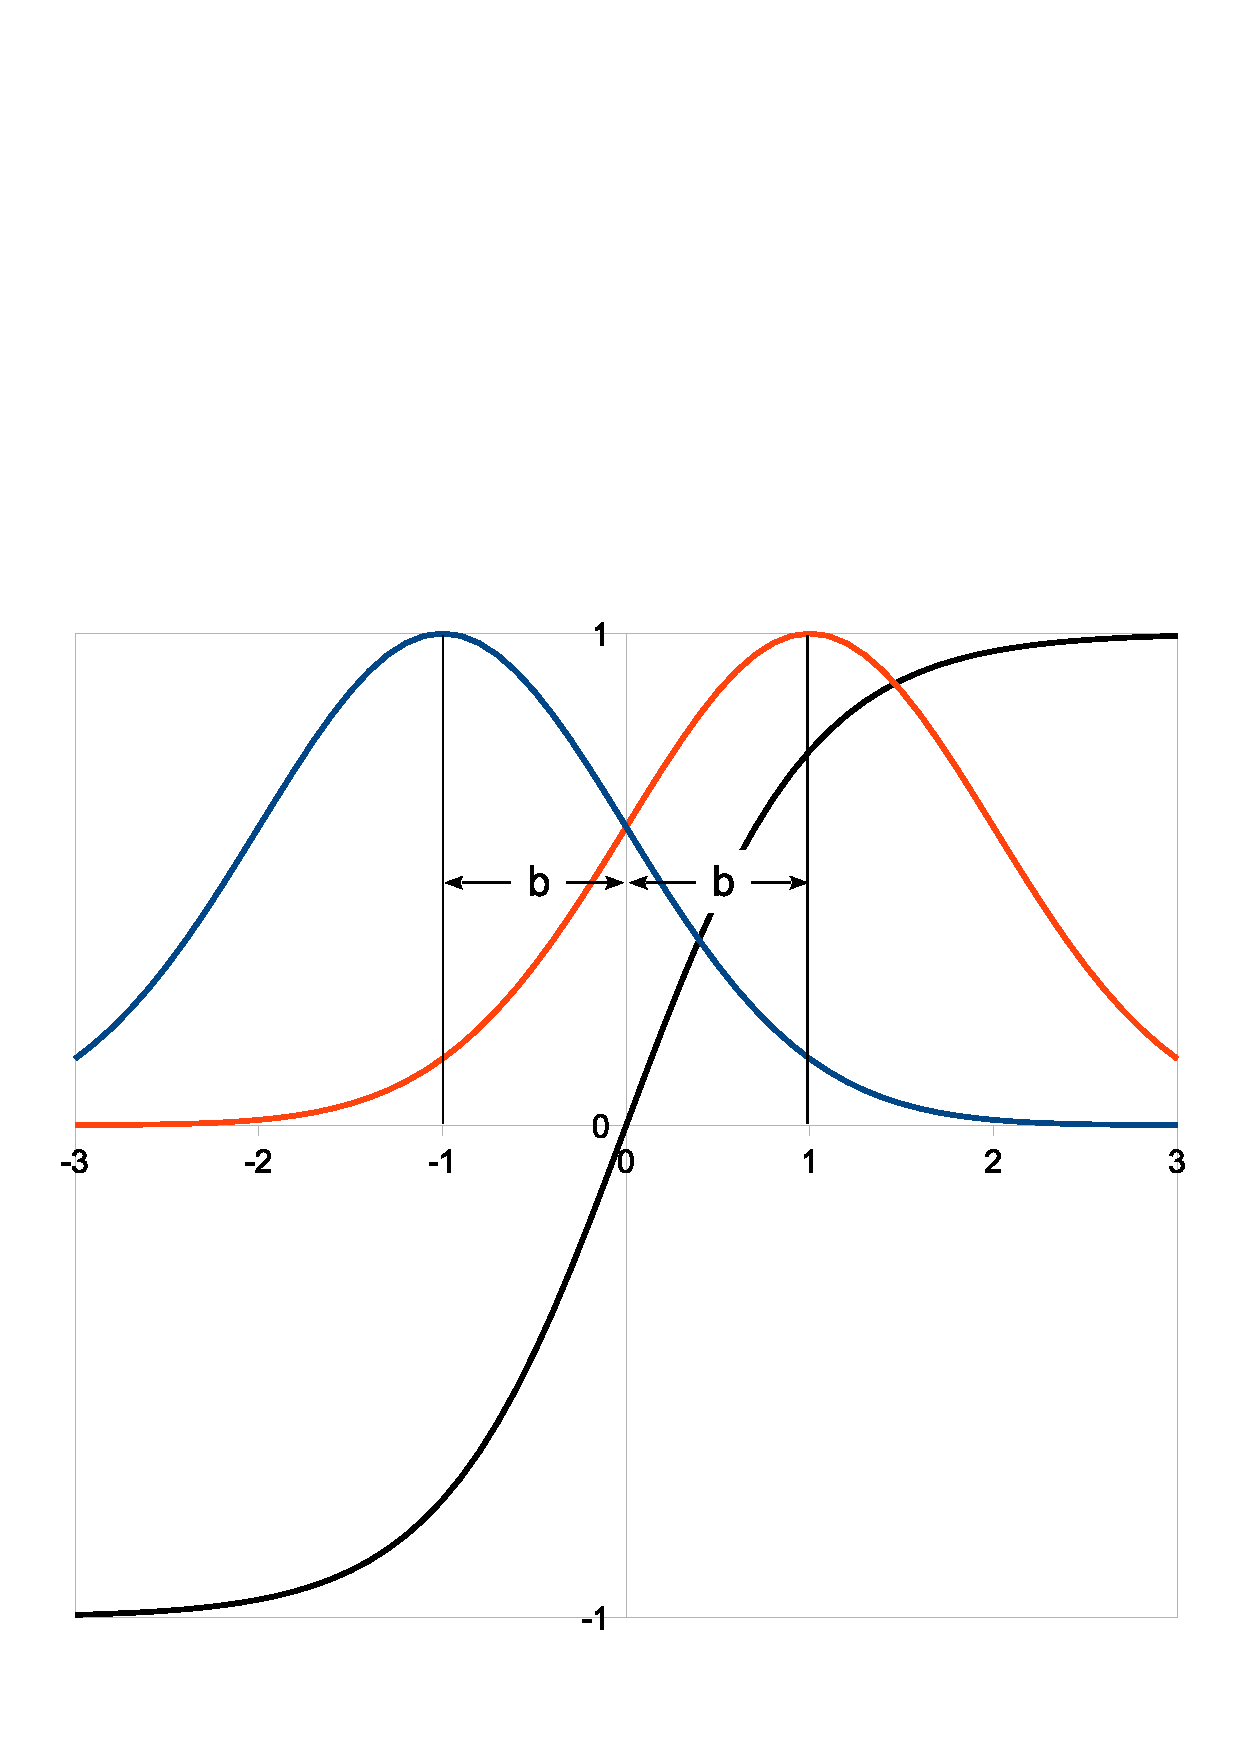
\includegraphics[width=0.9\textwidth]{logistic1}
	\caption{A one-dimensional model of binary classification comprised of a pair of identical Gaussian functions.}
	\label{model}
\end{figure}

Consider a pair of equally-sized, one-dimensional Gaussian functions of 
equal width, $h$, and spaced an equal distance, $b$, from the origin.
The difference in conditional probabilities is given:
\begin{eqnarray}
	R(x) & = & \frac{P(x,\,+1) - P(x,\,-1)}{P(x,\,-1)+P(x,\,+1)} \label{oned1}\\
	     & = & \frac{\exp \left [ -\frac{(x+b)^2}{2 h^2} \right ] - \exp \left [ -\frac{(x-b)^2}{2 h^2} \right ] }{\exp \left [ -\frac{(x+b)^2}{2 h^2} \right ] + \exp \left [ -\frac{(x-b)^2}{2 h^2} \right ]}
\end{eqnarray}
which, with some manipulation, works out to:
\begin{eqnarray}
	R(x) & = & \frac{\exp (b x/h) - \exp (- b x/h)}
	{\exp(b x/h) + \exp(-b x/h)}\\
		& = & \tanh (b x/h)
	\label{logistic_1d}
\end{eqnarray}
In other words, for a pair of equal-size Gaussians, the decision function
in one dimension is a hyperbolic tangent.

This may seem like a trivial example, however the $\tanh$ function is found
throughout the field of machine machine learning.
In statistical classification, it is often used to correct the decision
function to better estimate the conditional probabilities.
This is applied in the LIBSVM library, for instance, as well as in my own
machine learning library, libAGF.
The example illustrates why: the difference in conditional probabilities, $R$,
is, more often than not, sigmoidal close to the class borders.

Consider logistic regression. In logistic regression, we are fitting the
following decision function:
\begin{equation}
	f(\vec x) = \tanh (\vec v \cdot \vec x + a)
	\label{logistic}
\end{equation}
where $\vec v$ is a vector and $a$ a constant.
The fitting is performed by minimizing a cost function, for instance a least squares:
\begin{equation}
	\min_{\vec v, a} \sum_i \left [y_i - \tanh(\vec v \cdot \vec x_i + a)\right ]^2
	\label{logistic_fit}
\end{equation}
To fit or ``train'' the thing, we need some training data.
This comprises a set of ordered
pairs of a vector in the feature space mapping on to its corresponding 
class value: $\lbrace \vec x_i:y_i \rbrace$.
Here, $y_i$ takes on one of two values: -1 or +1, that is
$y_i \in \lbrace -1,\, +1 \rbrace$.

The training data represents the ``ground truth'' and could be obtained in
a variety of ways.
Consider a land classification problem: 
a satellite instrument measures upwelling electromagnetic radiation in several
bands and
on this basis, we are interested in classifying the
surface type, whether field, forest, city, or water, for instance.
The data could have been pain-stakingly measured by hand: an aircraft
carried a terrestial version of the instrument aloft and measured radiances
while observers in the craft noted the type of land they were flying over.
It could have been modelled: perhaps we have an algorithm that we trust that
returns modelled radiances depending on different parameters describing the
land surface.
In this case, the resulting training data is potentially infinite, although
not necessarily all that accurate.
Or perhaps it was measured by the actual instrument but classified by hand.
You have a simple app that brings up an image and each pixel can be classified
with a mouse click on the basis of color.

Equations (\ref{logistic}) and (\ref{logistic_fit}) provide a succinct
illustration of the entire process of statistical classification.
There is a training phase, given by (\ref{logistic_fit}), in which a model is
derived.
In this case the model consists of a small set of function parameters which
makes this an exercise in {\it parametric statistics}.
Contrast this with a {\it non-parametric} statistical model such as KNN
 which uses all of the training data for each classification.
For the logistic classifier, the fitting will be nonlinear, another common technique in machine learning.
Nonlinear optimization is normally performed with an iterative, numerical
algorithm, assuming the problem cannot be reduced to a closed-form, analytic
solution.
It is in itself a broad and diverse field, so we won't
go into the exact details.
See the problem set for more info.
The model is then applied to classify a series of test points using
Equation (\ref{logistic}).

\section{Calibration}

The nice thing about using a continuous decision function for binary
classification is that it allows some degree of calibration.
Consider the following classifier:
\begin{equation}
	c(\vec x) = \left \lbrace \begin{array}{rl}
		-1 & f(\vec x) < f_0 \\
		+1 & f(\vec x) > f_0
	\end{array} \right .
\end{equation}
Varying the classification threshold, $f_0$, 
allows us to adjust the sensitivity of the classifier.
This is particularly useful in medical diagnostics.
(Note that the case $f=f_0$ is left undefined. 
To remove bias,
a random value should be returned
when this occurs in numerical computations
.) 

Suppose the classifier is trained using data with a prior class distribution of
$P^\prime(i)$ while the population distribution is actually $P(i)$.
Assuming that $f$ accurately estimates $R$, 
we want to find the value for $f_0$ such that the sample statistics
are corrected to those of the population:
\begin{equation}
	f_0 = \frac{P^\prime(+1) P(-1) - P^\prime(-1) P(+1)}
	{P^\prime(+1) P(-1) + P^\prime(-1) P(+1)}
	\label{class_size_cal}
\end{equation}

\begin{figure}
	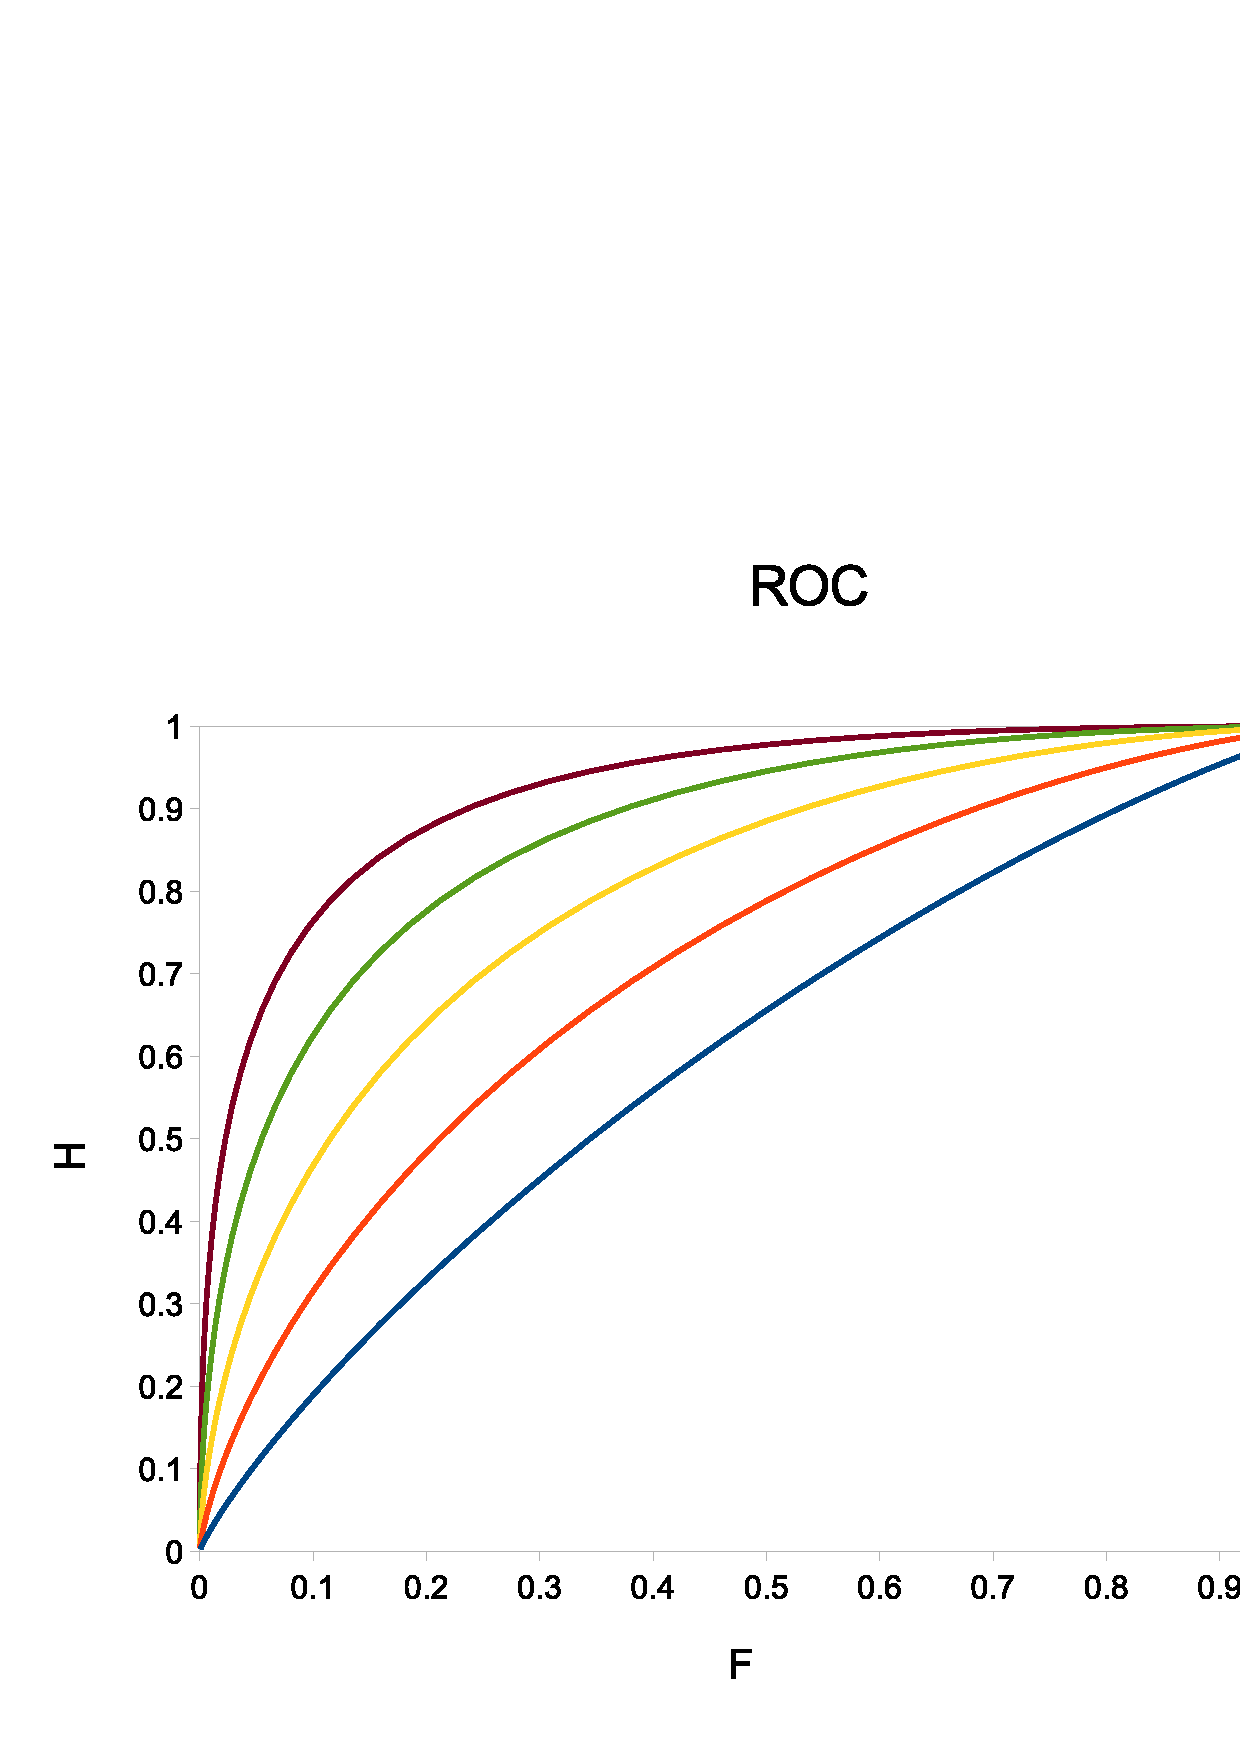
\includegraphics[width=0.9\textwidth]{roc}
	\caption{Receiver operating characteristic curves for the 1-D classification model in Figure \ref{model}}.
	\label{ROC}
\end{figure}

To make this more detailed, consider the confusion matrix.
The element of the confusion matrix in the $i$th row and $j$th column tells
us, for all of the test data, how many test samples had the $i$th class but the
classifier returned the $j$th class.
By dividing by the number of test samples, the confusion matrix can be
expressed as an approximate joint probability.
Consider the confusion matrix for a binary classifier:
\begin{equation}
	n_t \left [ \begin{array}{ll}
			p_{-1,-1} & p_{-1,+1} \\
			p_{+1,-1} & p_{+1,+1}
		\end{array} \right ]
		\approx
		\left [ \begin{array}{ll}
				n_{TN} & n_{FP} \\
				n_{FN} & n_{TP}
		\end{array} \right ]
\end{equation}
where:
\begin{itemize}
	\item $n_t=n_{TN}+n_{FP}+n_{FN}+n_{TP}$ is the total number of test samples
	\item $n_{TN}$ is the number of true negatives
	\item $n_{FP}$ is the number of false positives
	\item $n_{FN}$ is the number of false negatives
	\item $n_{TP}$ is the number of true positives
\end{itemize}
A perfect classifier would return a diagonal matrix: 
an element is non-zero only when $i=j$.
From these five parameters, you can write down all possible skill scores
for a simple binary classifier.
The receiver operating characteristic (ROC) curve is produced by plotting
two such skill scores against one another while varying the classification
threshold.
These are the hit rate:
\begin{equation}
	H = \frac{n_{TP}}{n_{TP} + n_{FN}}
\end{equation}
and the false alarm rate:
\begin{equation}
	F = \frac{n_{FP}}{n_{TP} + n_{FP}}
\end{equation}
Figure \ref{ROC} plots the ROC curve for the one-dimensional logistic classifier
in (\ref{logistic_1d}) for $h=1$ and for different values of $b$.
The classifier is assumed to be a perfect estimator for the conditional
probabilities.

A more sophisticated calibration exercise would transform the decision
function such that it accurately represents the difference in conditional
probabilities.
Consider the following equation, derived strictly from the background material
presented in the first two sections:
\begin{equation}
%\lim_{n \rightarrow \infty} \left \lbrace n = \sum_{i=1}^n \frac{\delta_{c y_i}}{P(c | \vec x_i)} \right \rbrace
\lim_{n \rightarrow \infty} \sum_{i=1}^n \left \lbrace P(c | \vec x_i) - \delta_{c y_i} \right \rbrace = 0
\label{full_cal}
\end{equation}
where $\delta$ is the Dirac delta function:
\begin{equation}
	\delta_{ij} = \left \lbrace \begin{array}{rl}
		1 & i = j \\
		0 & i \ne j
	\end{array} \right .
\end{equation}
A well-calibrated estimator for the conditional probabilities should obey this
equation.

\section{Validation}

Once we have derived a statistical classifier, we need to validate it on
some test data.
This data should be different from that used to train the classifier otherwise
skill scores will be unduly optimistic.
The confusion matrix expresses everything about 
the accuracy of a discrete classifier over a given datase and you can use it
to compose any possible skill score.
Here we are going to cover two that are rarely seen in the literature but are
nonetheless important for reasons that will become clear.

The first is the uncertainty coefficient.
This measure is based on Shannon's channel capacity and requires, first, a
definition of the information entropy.
For a discrete probability, this is:
\begin{equation}
	H_i = - \sum_i P_i \log P_i
\end{equation}
and tells us how many bits we need to represent $i$ given
that its prior distribution is $P_i$.
The measure can be extended to multi-variate distributions.
The conditional entropy is given:
\begin{equation}
	H(i|j) = - \sum_{i,\,j} P_{ij} \log P(i|j)
\end{equation}
Once we have these two definitions out of the way, we can write down the
uncertainty coefficient:
\begin{equation}
	U(i|j) = \frac{H_i - H(i|j)}{H_i}
\end{equation}
which tells us how many bits of information a single classification gives us
of the true class value, $i$.
This makes it a good skill score since the lowest possible value is 0 meaning
the classifier provides, on average, no information on the true class value
while the highest is 1 meaning the classifier provides full information.
Contrast this with accuracy which, for completeness, we write down:
\begin{equation}
	A = \frac{n_{TP}}{n_t}
\end{equation}
even though I don't recommend using this measure.

For binary classifiers, I also recommend the Pearson correlation coefficient:
\begin{equation}
	r= \frac{n_{TN} n_{TP} - n_{FN} n_{FP}}
	{\sqrt{(n_{TP} + n_{FP}) (n_{TN} + n_{FN})(n_{TP} + n_{FN}) (n_{FP} + n_{TN})}}
	\label{correlation}
\end{equation}
which has many similar properties to the uncertainty coefficient.

Finally, for binary classifiers that return a continuum decision function
rather than a discrete, binary value,
we can use
the ROC curve to measure the average skill for all possible thresholds by calculating
the area under the curve.
For a perfect classifier, the ROC curve will follow the unit square, rising
to $H=1$ at $F=0$ and staying there for the duration, thus the area will
be 1.
An area of 0 is also a perfect classifier, but the sign is reversed, while
a classifier with no discrimination value will follow the diagonal 
with an area of 0.5.
Note for instance, how the area under the example curves gets larger as the separation between the classes increases.

\section{Multi-class classification}

We have spent a considerable amount of time discussing binary classifiers.
Assuming the only suitable statistical classifier we have at our disposal is a 
binary classifier, how do we generalize it to 
classification problems with more than two classes,
that is, multi-class classifiers?
We can use probability theory to derive an answer.

Suppose we design a set of binary classifiers by
multiply partitioning the classes into two sets.
A coding matrix, $A$, describes how this partitioning is done:
the $i$th row of the matrix describes the partitioning of the $i$th
binary classifier with a $-1/+1$ in the $j$th column meaning that the $j$th
class label was transformed to a $-1/+1$ for the training 
%while a $1$ meaning it was transformed to a $+1$ 
and a $0$ meaning it was excluded entirely.
The conditional probabilities of the multiclass problem 
are related to those of the binary classifiers as follows:
\begin{equation}
	R_i (\vec x) = \frac{\sum_j a_{ij} P(j | \vec x)}
	{\sum_j | a_{ij} | P(j | \vec x)}
	\label{multiclass1}
\end{equation}
With some rearrangement, we can transform this into a linear system:
\begin{equation}
	\sum_j \left [ a_{ij} + (1 - |a_{ij}|) R_i \right ] P(j | \vec x) = R_i
	\label{multiclass2}
\end{equation}
where $R_i$ is the difference in conditional probability for the $i$th binary
classifier.

As an example, consider the ``one-versus-the-rest'' approach to multi-class
classification.
Here we compare each class with all the others.
The coding matrix is given:
\begin{equation}
	a_{ij} = \left \lbrace \begin{array}{rl}
		1 & i = j \\
		-1 & i \ne j
	\end{array} \right .
	\label{onevr}
\end{equation}

The above assumes that the conditional probabilities for the binary classifiers
are estimated correctly.
Otherwise we need to constrain the resulting multi-class probabilities.
Neglecting the second argument, 
a conditional probability has the same properties as a univariate probability.
First, they ought to sum to one:
\begin{equation}
	\sum_j P(j|\vec x) = 1
	\label{norm}
\end{equation}
Second, they should all be positive:
\begin{equation}
	P(j|\vec x) \ge 0
\end{equation}

The normalization constraint in (\ref{norm}), being an equality constraint,
is the easiest to enforce.
One way is to introduce a ``slack'' variable:
\begin{eqnarray}
	\sum_j q_{ij} P(j|\vec x) + \lambda & = & b_i \nonumber \\
	\sum_j P(j|\vec x) & = & 1 \label{symmetric_norm}
\end{eqnarray}
where $Q \vec p = \vec b$ is the linear system for the unconstrained problem
and $\lambda$ is a ``slack'' variable.

For the ``one-versus-one'' method of multi-class classification, where we
compare each class with each of the others in turn, this is all we need.
It turns out that once the normalization constraint is enforced, all the others
fall into place and the solution has only positive elements.
Note that because the system of equations is over-determined, 
it will need to be solved as a least-squares problem and there is one
other caveat: the normalization must be done separately from the least
squares minimization.
In other words, we form the normal equations from (\ref{multiclass2}) first,
then plug these into (\ref{symmetric_norm}).

\section{Conclusion}

Mathematical models are not closed systems. They can be expanded, re-purposed, and recombined.
The applications of probability and Bayes� theorem and the problems we can put them to are limited only by the imagination. Here we have presented just a few of the ways to use these tools to help gain a foothold in the complex world of computational learning algorithms.

\section{Problems}

\begin{enumerate}
	\item Why does the fitting for the logistic classifier in (\ref{logistic}) have to be nonlinear? What advantage does this have?
	\item Do some research online to find lonlinear optimization algorithms to fit the logistic classifier.
	\item What is the major disadvantage of the logistic classifier?
	\item Derive Equation (\ref{class_size_cal}). (It's surprisingly difficult.) How important do you think it is, on average, to correct for the class distribution? Explain.
	\item How would you calculate the ROC curves in Figure \ref{ROC}? Fill in the missing steps going from Equation (\ref{decision}) to (\ref{oned1}) to (\ref{logistic_1d}) and then to calculation of the ROC curves.
	\item Derive Equation (\ref{full_cal}).
	\item List the advantages of the uncertainty coefficient and the correlation coefficient (for binary classifiers) as a measure of classification skill.
	What happens when 
	a) the class labels are rearranged and 
	b) the distribution of the class labels is changed in the test data? 
	How does this affect the outcome?
	\item From the general formula for Pearson correlation, derive Equation (\ref{correlation}). Note: this is not trivial.
	\item Correlation is normally not appropriate for multi-class classification problems. Why not? What types of problem would be the exceptions?
	\item Derive Equation (\ref{multiclass2}) from Equation (\ref{multiclass1}). 
	Hint: what property of $P(i|\vec x)$ do you need to complete the derivation?
	\item The one-versus-the-rest coding matrix in (\ref{onevr}) can use a simpliefied version of Equation (\ref{multiclass2}). Explain.
	\item Write down the coding matrix for the one-versus-one multi-class classifier.
	\item Find some statistical classification data online or create some on your own, e.g., by classifying pixels in an image.
		Perform statistical classifications by fitting a multi-dimensional Gaussian to each of the classes:
		\begin{equation}
			P(\vec x | i) \approx \frac{1}{\sqrt{(2 \pi)^D |\Sigma|}}
				\exp \left [ - (\vec x - \vec \mu) \Sigma (\vec x - \vec \mu) \right ]
			\end{equation}
			where $\Sigma$ is the covariance matrix, $\vec \mu$ is the arithmetic mean and $D$ is the dimension of the features data. Measure the accuracy of your results. Don't forget to divide the data into a test set and a training set.
\end{enumerate}

\end{document}
